\documentclass[11pt]{article}
\usepackage{myz310e-notes}
\renewcommand{\topfraction}{0.85}\renewcommand{\textfraction}{0.1}\renewcommand{\floatpagefraction}{0.8}
% compact pseudocode in this note: indentation shows the block structure, so the "end" lines are omitted
\algtext*{EndFor}\algtext*{EndIf}\algtext*{EndFunction}\algtext*{EndWhile}
\newcommand{\toy}[1]{\textsf{P#1}}% the ten points of Table 1
\hypersetup{pdftitle={Histogram methods and the curse of dimensionality},pdfauthor={Emre Onur Kahya},pdfsubject={MYZ 310E Machine Learning in Physics, Fall 2026, lecture note 3 (week 2)}}

\begin{document}
\NoteTitle{3}{2}{Histogram methods and\\ the curse of dimensionality}{Histograms and the curse}{%
The simplest learning algorithm cuts the input space into cells and counts. It solves all three tasks of Note~1 ---
classification, regression and density estimation --- works well in one or two dimensions, and fails completely in
ten. This note trains histograms by hand on small datasets, writes the three algorithms in pseudocode with their
running times, and derives the bias and variance of a histogram and the best bin width. It then quantifies the
\emph{curse of dimensionality} --- empty cells, neighbourhoods that are not local, volume near the boundary,
distances that all look alike --- and explains the ideas that modern methods use to escape it: adaptive partitions
such as decision trees, low intrinsic dimension and learned representations. The note also walks through the steps
of designing and analysing an algorithm.}

\section{Cut the space into cells and count}\label{sec:hist}

\paragraph{Where we start} The setting is that of Note~1: a training set of $n$ examples, each a feature vector in
$\R^d$ with a target, drawn i.i.d.\ from an unknown distribution (Note~1, Section~2, which also lists datasets that
break this assumption); the three task families, the kind of function each one searches for and their losses
(Note~1, Section~4 and Table~2); and the steps of a machine-learning project, from formulating the task to
deployment and monitoring (Note~1, Section~5). Section~\ref{sec:design} below adds the steps of designing an algorithm to that list.

\paragraph{Notation} In this note $m$ always denotes the number of bins per axis, as in the lectures. We therefore
write $K$ for the number of classes (Note~1 calls it $m$). The other symbols are those of Note~1: $n$ training
examples, $d$ features.

Suppose we want $\E[Y \mid \x]$, a class probability or a density at a point $\x$ where we have no measurement. The
data say nothing about $\x$ itself, so information must be borrowed from somewhere; the crudest source is a fixed
box around $\x$. Cover the input space with boxes, or cells, $C_1, \dots, C_M$, and summarise the training points
of each cell by one number. With $m$ equal bins along each of $d$ axes the cells are boxes of side $h$ and there
are $M = m^d$ of them. Write $C(\x)$ for the cell containing $\x$ and $n_C$ for the number of training points in
cell $C$. One rule then serves each task of Note~1, Table~2:

\begin{center}\small
\begin{tabular}{@{}L{0.17\linewidth}L{0.4\linewidth}L{0.35\linewidth}@{}}
\toprule
Task & Prediction at $\x$ & Interpretation \\
\midrule
Classification & majority label among the points in $C(\x)$ & estimate of $P(Y = k \mid \X \in C(\x))$ by class frequencies \\
Regression & average of $y_i$ over the points in $C(\x)$ & estimate of $\E[Y \mid \X \in C(\x)]$ \\
Density & $\hat p(\x) = \dfrac{n_{C(\x)}}{n\,\mathrm{vol}(C(\x))}$ & fraction of the data per unit volume \\
\bottomrule
\end{tabular}
\end{center}

All three rules replace the unknown conditional quantity at $\x$ by its average over a neighbourhood --- here, the
cell. The neighbourhood is fixed in advance, which is both the simplicity and the weakness of the method; Note~5
centres the neighbourhood on the query point instead.

\subsection{Cells, counts and the three estimators}\label{sec:formulas}

\paragraph{Which cell} Choose a box $[a_1, b_1] \times \dots \times [a_d, b_d]$ that contains the data and cut each
side into $m$ equal bins of width $h_j = (b_j - a_j)/m$. Coordinate $x_j$ falls in bin
\begin{equation}\label{eq:binindex}
  c_j(\x) = \Big\lfloor \frac{x_j - a_j}{h_j} \Big\rfloor \in \{0, 1, \dots, m - 1\},
\end{equation}
where $\lfloor\cdot\rfloor$ rounds down (points exactly on the upper edge $b_j$, or outside the box, are clipped to
the nearest bin). The cell $C(\x)$ of $\x$ is the box whose index is the tuple $(c_1, \dots, c_d)$; we use the same symbol for the
box (as in $\x_i \in C$) and for its index tuple (as in the arrays of the algorithms). Its volume is
$h_1 h_2 \cdots h_d$, or $h^d$ when all widths are equal. Computing the tuple costs $d$ subtractions, divisions and
roundings. Nothing forces the same number of bins on every axis: with $m_j$ bins along axis $j$ there are
$M = m_1 m_2 \cdots m_d$ cells, and every $m^d$ below becomes this product. Classification and regression clip a
point outside the box to the nearest edge cell, so that every query receives a prediction; the density estimate
instead returns 0 outside the box, because the cells only cover the box and a point outside it lies in none of
them.

\paragraph{Counts} Training only counts. For every cell $C$ and class $k$ let
\[
  N_{C,k} = \#\{i : \x_i \in C,\ y_i = k\}, \qquad n_C = \sum_{k=1}^K N_{C,k} = \#\{i : \x_i \in C\} .
\]
These counts are the \emph{parameters} of the model: they are computed from the data. The number of bins and the
box are \emph{hyperparameters}: they are fixed before counting.

\paragraph{Classification} The class frequencies in the cell estimate the class probabilities, and the prediction
is the most frequent class:
\begin{equation}\label{eq:classprob}
  \hat P(Y = k \mid \x) = \frac{N_{C(\x),k}}{n_{C(\x)}}, \qquad f(\x) = \argmax_k N_{C(\x),k} .
\end{equation}
The majority vote is not arbitrary: if the cell predicts class $k$, its training errors are the $n_C - N_{C,k}$
points of the other classes, and this number is smallest for the class with the largest count. The majority vote
therefore minimises the training error inside every cell.

\paragraph{Regression} The prediction in cell $C$ is the constant $\hat y_C$ that minimises the squared error of the
points of that cell. Write $J(w) = \sum_{i : \x_i \in C} (y_i - w)^2$ for a constant prediction $w$. Setting the derivative to zero,
\[
  \frac{dJ}{dw} = -2 \sum_{i : \x_i \in C} (y_i - w) = 0
  \quad\Longrightarrow\quad n_C\, w = \sum_{i : \x_i \in C} y_i
  \quad\Longrightarrow\quad \hat y_C = \frac{1}{n_C} \sum_{i : \x_i \in C} y_i ,
\]
and $d^2J/dw^2 = 2 n_C > 0$ confirms a minimum. The cell mean is the empirical version of $\E[Y \mid \X \in C]$, which
Note~1, Section~4, showed to be the best prediction under squared error.

\paragraph{Density} The estimate $\hat p(\x) = n_{C(\x)} / (n\,\mathrm{vol}(C(\x)))$ is a valid density. It is
non-negative, and because it is constant on each cell,
\[
  \int \hat p(\x)\, d\x = \sum_C \int_C \frac{n_C}{n\,\mathrm{vol}(C)}\, d\x
  = \sum_C \frac{n_C}{n\,\mathrm{vol}(C)}\, \mathrm{vol}(C) = \sum_C \frac{n_C}{n} = \frac{n}{n} = 1 .
\]
It is also the maximum-likelihood estimate among all densities that are constant on the cells: with
$\theta_C = P(\X \in C)$ the likelihood is that of a categorical distribution over the cells, whose maximum is at
$\theta_C = n_C/n$ (Note~2, Section~2; Question~C2 below). Note that $\hat p = 0$ outside the box and in every empty cell: a test point there has log-likelihood
$-\infty$, the worst possible value of the loss $-\log \hat p(\x)$.

\paragraph{Empty cells} A cell with $n_C = 0$ gives no information, and \eqref{eq:classprob} becomes $0/0$. Any
implementation must choose a \emph{fallback}: predict the overall majority class (or the overall mean of $y$),
borrow the prediction of the nearest occupied cell, merge with neighbouring cells, or refuse to predict. All of these
are patches; Section~\ref{sec:curse} shows that in high dimension almost every query needs the patch.

\begin{table}[h]\centering\small
\caption{Ten labelled points in $[0,3]^2$ used in the worked examples ($y = 1$: signal, $y = 0$: background).}
\label{tab:toy}
\begin{tabular}{@{}l*{10}{c}@{}}\toprule
point & \toy{1} & \toy{2} & \toy{3} & \toy{4} & \toy{5} & \toy{6} & \toy{7} & \toy{8} & \toy{9} & \toy{10} \\ \midrule
$x_1$ & 0.6 & 0.3 & 1.4 & 1.7 & 2.5 & 1.5 & 2.1 & 2.4 & 2.7 & 2.8 \\
$x_2$ & 1.2 & 1.7 & 0.5 & 1.3 & 0.4 & 2.4 & 2.3 & 2.7 & 2.3 & 2.1 \\
$y$   & 0 & 0 & 0 & 0 & 0 & 1 & 1 & 1 & 1 & 0 \\ \bottomrule
\end{tabular}
\end{table}

\begin{worked}{a histogram classifier by hand}
Use the ten points of Table~\ref{tab:toy} (six of class 0, four of class 1) and bins of width 1 on $[0, 3]$ along
each axis.

\textbf{One feature.} With $x_1$ only there are three bins:

\begin{center}\small
\begin{tabular}{@{}lllccc@{}}\toprule
bin of $x_1$ & points & $(N_0, N_1)$ & $\hat P(Y = 1 \mid \text{bin})$ & prediction & training errors \\ \midrule
$[0, 1)$ & \toy{1}, \toy{2} & $(2, 0)$ & $0$ & 0 & 0 \\
$[1, 2)$ & \toy{3}, \toy{4}, \toy{6} & $(2, 1)$ & $1/3$ & 0 & 1 (\toy{6}) \\
$[2, 3)$ & \toy{5}, \toy{7}--\toy{10} & $(2, 3)$ & $3/5$ & 1 & 2 (\toy{5}, \toy{10}) \\ \bottomrule
\end{tabular}
\end{center}
The training error is $3/10$. Every bin is occupied, but the second and third bins mix both classes.

\textbf{The other feature.} With $x_2$ only, the bins $[0, 1)$, $[1, 2)$ and $[2, 3)$ hold \toy{3}, \toy{5} with
counts $(2, 0)$; \toy{1}, \toy{2}, \toy{4} with $(3, 0)$; and \toy{6}--\toy{10} with $(1, 4)$. They predict 0, 0
and 1, and only \toy{10} is misclassified: training error $1/10$ with three bins and none empty. A single feature
can be far more informative than another one.

\textbf{Two features.} With both features there are $3 \times 3 = 9$ cells. The table below is drawn like the plane
($x_2$ increases upwards); each entry lists the points and the counts $(N_0, N_1)$:

\begin{center}\small
\begin{tabular}{@{}l|ccc@{}}
$x_2 \in [2, 3)$ & empty $(0, 0)$ & \toy{6} $(0, 1)$ & \toy{7}--\toy{10} $(1, 3)$ \\
$x_2 \in [1, 2)$ & \toy{1}, \toy{2} $(2, 0)$ & \toy{4} $(1, 0)$ & empty $(0, 0)$ \\
$x_2 \in [0, 1)$ & empty $(0, 0)$ & \toy{3} $(1, 0)$ & \toy{5} $(1, 0)$ \\ \hline
 & $x_1 \in [0, 1)$ & $x_1 \in [1, 2)$ & $x_1 \in [2, 3)$
\end{tabular}
\end{center}
Only \toy{10} is misclassified, so the training error drops from the $3/10$ of $x_1$ alone to $1/10$. But six cells hold the ten points, three cells
are empty, and four of the occupied cells contain a single point (Figure~\ref{fig:toy}, left).

\textbf{Predictions.} The overall majority class is 0 (six against four); it is the fallback for empty cells.
\begin{itemize}
\item $q_1 = (2.5, 1.5)$ lies in the empty cell $[2,3) \times [1,2)$, so the 2-D classifier falls back to class 0.
The 1-D classifier puts $q_1$ in the bin $[2, 3)$ and predicts class 1 with $\hat P = 3/5$.
\item $q_2 = (1.2, 2.8)$ lies in the cell of \toy{6} alone: class 1 with $\hat P(Y = 1) = 1/1 = 1$ --- a certainty based on
a single example. The 1-D classifier predicts class 0 with $\hat P(Y = 1) = 1/3$.
\item $q_3 = (2.75, 2.75)$ lies in the cell of \toy{7}--\toy{10}: class 1 with $\hat P(Y = 1) = 3/4$.
\end{itemize}
Adding $x_2$ to $x_1$ lowers the training error, but four of the six occupied cells now rest on a single point, and
the prediction at $q_1$ is decided by the fallback rule rather than by the data. Yet $x_2$ alone reached the same
training error with three occupied bins: choosing the right feature matters as much as adding features. A decision
tree (Section~\ref{sec:trees}) makes this choice from the data.
\end{worked}

\begin{figure}[h]
\centering
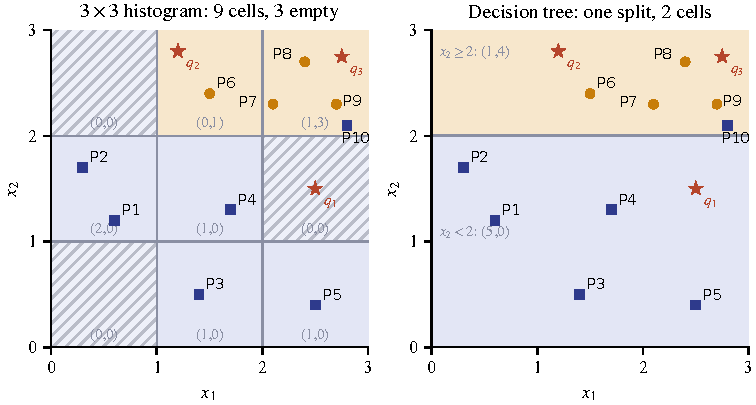
\includegraphics[width=0.8\linewidth]{figures/n3_toy.pdf}
\caption{The ten points of Table~\ref{tab:toy} (squares: class 0, circles: class 1) and three queries (stars).
Left: the $3 \times 3$ histogram classifier; shading is the predicted class, counts are $(N_0, N_1)$, hatched cells are
empty and fall back to class 0. Right: a decision tree with a single split at a grid line (Section~\ref{sec:trees})
reaches the same training error with two cells and no empty cell.}
\label{fig:toy}
\end{figure}

\begin{worked}{histogram density values}
Estimate the density of $x_1$ from the ten values of Table~\ref{tab:toy}: $0.3, 0.6, 1.4, 1.5, 1.7, 2.1, 2.4, 2.5,
2.7, 2.8$.
\begin{itemize}
\item Width $h = 1$ (bins $[0,1), [1,2), [2,3)$): counts $2, 3, 5$, so $\hat p = 2/(10 \cdot 1) = 0.2$,
$3/10 = 0.3$ and $5/10 = 0.5$. At $x = 2.45$ the estimate is $0.5$. Check: $(0.2 + 0.3 + 0.5) \times 1 = 1$.
\item Width $h = 0.5$ (six bins): counts $1, 1, 1, 2, 2, 3$, so $\hat p = n_C/(10 \times 0.5) = 0.2, 0.2, 0.2, 0.4,
0.4, 0.6$. At $x = 2.45$ (bin $[2, 2.5)$) the estimate is now $0.4$. Check: $(0.2 + 0.2 + 0.2 + 0.4 + 0.4 + 0.6)
\times 0.5 = 1$.
\end{itemize}
In two dimensions with unit cells, the density at $q_3$ is $\hat p(q_3) = 4/(10 \times 1) = 0.4$ points per unit
area, while $\hat p(q_1) = 0$: the model declares a perfectly plausible point impossible (log-likelihood $-\infty$
if such a point is ever observed).
\end{worked}

\begin{worked}{histogram regression}
Eight calibration measurements relate a detector reading $x$ to a true energy $y$:

\begin{center}\small
\begin{tabular}{@{}l*{8}{c}@{}}\toprule
$x$ & 0.2 & 0.7 & 1.1 & 1.4 & 1.8 & 3.1 & 3.5 & 3.9 \\
$y$ & 1.0 & 1.4 & 2.1 & 2.5 & 2.3 & 4.6 & 5.2 & 4.9 \\ \bottomrule
\end{tabular}
\end{center}

\textbf{Bins of width 1 on $[0, 4)$.} The bin means are $\hat y = (1.0 + 1.4)/2 = 1.2$ on $[0,1)$,
$(2.1 + 2.5 + 2.3)/3 = 2.3$ on $[1,2)$, and $(4.6 + 5.2 + 4.9)/3 = 4.9$ on $[3,4)$; the bin $[2,3)$ is empty. The
residuals $y_i - \hat y$ are $-0.2, 0.2, -0.2, 0.2, 0, -0.3, 0.3, 0$, so the training mean squared error is
$0.34/8 = 0.0425$. At $x = 2.5$ we need a fallback: the overall mean $24.0/8 = 3.0$, or the average of the two
neighbouring bins, $(2.3 + 4.9)/2 = 3.6$.

\textbf{Bins of width 2.} The means are $9.3/5 = 1.86$ on $[0, 2)$ and $4.9$ on $[2, 4)$; there is no empty bin and
$f(2.5) = 4.9$. The residuals $-0.86, -0.46, 0.24, 0.64, 0.44, -0.3, 0.3, 0$ give a training mean squared error of
$1.792/8 = 0.224$. Narrower bins fit the training data better; whether they predict new data better is a question for
held-out data (Note~4).

\textbf{More inputs.} With two or more inputs nothing changes except that the bins become cells indexed by tuples:
each cell predicts the mean target of its points, and an empty cell needs the same fallback.
\end{worked}

\subsection{The three algorithms in pseudocode}\label{sec:pseudo}

The three estimators share the cell index \eqref{eq:binindex} and differ only in what is accumulated per cell:
class counts (Algorithm~\ref{alg:hist}), sums of targets or plain counts (Algorithm~\ref{alg:histreg}). The arrays are \emph{dense}: one entry for each of the $m^d$ cells, indexed by the
tuple $(c_1, \dots, c_d)$. Section~\ref{sec:design} replaces them by a hash table.

\begin{algorithm}[H]
\caption{Histogram classifier with $m$ bins per axis on the box $[a_1, b_1] \times \dots \times [a_d, b_d]$}
\label{alg:hist}
\small
\begin{algorithmic}[1]
\Require hyperparameters $m$, $(a_j, b_j)_{j=1}^d$; training set $\Dtrain = \{(\x_i, y_i)\}_{i=1}^n$ with $K$ class labels, here numbered $1, \dots, K$ (in Table~\ref{tab:toy} the labels are 0 and 1)
\Function{CellIndex}{$\x$}
  \For{$j = 1, \dots, d$}
    \State $c_j \gets \min\big(m - 1,\; \max(0,\; \lfloor m (x_j - a_j)/(b_j - a_j) \rfloor)\big)$ \Comment{clip to the box}
  \EndFor
  \State \Return $(c_1, \dots, c_d)$
\EndFunction
\Function{Train}{$\Dtrain$}
  \State $N[c, k] \gets 0$ for every cell $c$ and class $k$ \Comment{$K m^d$ counters}
  \For{each $(\x_i, y_i) \in \Dtrain$}
    \State $c \gets \Call{CellIndex}{\x_i}$; \ $N[c, y_i] \gets N[c, y_i] + 1$
  \EndFor
  \State $\hat\pi_k \gets \frac{1}{n}\#\{i : y_i = k\}$ for $k = 1, \dots, K$ \Comment{fallback for empty cells, $O(n)$}
\EndFunction
\Function{ClassProb}{$\x$} \Comment{returns $(\hat P(Y = 1 \mid \x), \dots, \hat P(Y = K \mid \x))$}
  \State $c \gets \Call{CellIndex}{\x}$; \ $s \gets \sum_{k} N[c, k]$
  \If{$s = 0$} \Return $(\hat\pi_1, \dots, \hat\pi_K)$ \Comment{empty cell} \EndIf
  \State \Return $N[c, \cdot] / s$
\EndFunction
\Function{Predict}{$\x$}
  \State \Return $\argmax_k$ of \Call{ClassProb}{$\x$} \Comment{an empty cell gives the overall majority class}
\EndFunction
\end{algorithmic}
\end{algorithm}

\begin{algorithm}[H]
\caption{Histogram regression (\textsc{Reg}) and density estimation (\textsc{Dens}); both use \textsc{CellIndex} of Algorithm~\ref{alg:hist}}
\label{alg:histreg}
\small
\begin{algorithmic}[1]
\Require hyperparameters as in Algorithm~\ref{alg:hist}; training set with $y_i \in \R$ (regression) or unlabelled $\x_1, \dots, \x_n$ (density)
\Function{RegTrain}{$\Dtrain$}
  \State $S[c] \gets 0$, \ $N[c] \gets 0$ for every cell $c$ \Comment{sum of targets and count per cell}
  \For{each $(\x_i, y_i) \in \Dtrain$}
    \State $c \gets \Call{CellIndex}{\x_i}$; \ $S[c] \gets S[c] + y_i$; \ $N[c] \gets N[c] + 1$
  \EndFor
  \State $\bar y \gets \frac{1}{n} \sum_i y_i$ \Comment{fallback for empty cells}
\EndFunction
\Function{RegPredict}{$\x$}
  \State $c \gets \Call{CellIndex}{\x}$
  \If{$N[c] = 0$} \Return $\bar y$ \EndIf
  \State \Return $S[c] / N[c]$ \Comment{the cell mean}
\EndFunction
\Function{DensTrain}{$\x_1, \dots, \x_n$}
  \State $N[c] \gets 0$ for every cell $c$
  \For{$i = 1, \dots, n$}
    \State $c \gets \Call{CellIndex}{\x_i}$; \ $N[c] \gets N[c] + 1$
  \EndFor
  \State $\mathrm{vol} \gets \prod_{j=1}^d (b_j - a_j)/m$ \Comment{volume of one cell}
\EndFunction
\Function{Density}{$\x$}
  \If{$\x$ lies outside the box} \Return $0$ \EndIf
  \State \Return $N[\Call{CellIndex}{\x}] / (n \cdot \mathrm{vol})$
\EndFunction
\end{algorithmic}
\end{algorithm}

\begin{runtime}{histogram classifier, regression and density (dense arrays)}
Symbols: $n$ training points, $d$ features, $m$ bins per axis, $K$ classes, $M = m^d$ cells.
\begin{itemize}[leftmargin=1.2em]
\item \textbf{Training:} $O(KM + nd)$ for the classifier, $O(M + nd)$ for regression and density. The first term
initialises one counter per cell (and class); the second is one pass over the data with $O(d)$ work per point to
compute the cell index.
\item \textbf{Prediction per query:} $O(d + K)$ for the classifier ($d$ for the index, $K$ to find the largest
count); $O(d)$ for regression and density.
\item \textbf{Memory:} $O(KM)$ or $O(M)$ for the arrays --- exponential in $d$ --- plus the $K$ fallback frequencies
(or $\bar y$); the training set can be discarded after counting.
\item \textbf{In practice:} with NumPy the whole training is three vectorised calls (floor of an $n \times d$ array,
conversion of the tuples to flat indices, and \texttt{bincount}); this is still $O(nd + M)$ but runs in compiled
code. A GPU helps only for very large $n$: building a histogram with atomic additions is limited by memory
bandwidth, which GPUs have more of, but for the sizes of this course the single pass is faster than copying the data
to the device. Up to $M \approx 10^7$
cells ($d \le 3$ with $m \le 200$) dense arrays are perfectly practical.
\end{itemize}
\end{runtime}

\subsection{Density estimation in one dimension}

Figure~\ref{fig:histdens} shows the effect of the number of bins on a density estimate from 200 points. Too few bins
and the estimate is a coarse staircase that misses the structure (\emph{bias}); too many and most bins contain zero or
one point, so the estimate is dominated by the luck of the sample (\emph{variance}). The counts are random: $n_C$ is
binomial, and when $P(\X \in C)$ is small it is approximately Poisson with mean $\mu_C = n\,P(\X \in C)$. Its
standard deviation is then $\sqrt{\mu_C}$ and its relative fluctuation $1/\sqrt{\mu_C}$ --- the $\sqrt N$ error bar
physicists draw on every bin, with the observed count $N$ standing in for the unknown $\mu_C$. A bin expecting 4
counts is uncertain by about 50\%, a bin expecting 400 counts by about 5\%.

The training data alone cannot choose the number of bins. As $h \to 0$ every training point ends up alone in a tiny
bin, where $\hat p(x_i) = 1/(nh) \to \infty$, so the log-likelihood of the training data grows without bound while
almost every new point lands in an empty bin. The width must be judged on data not used for counting (Note~4), or
from a formula such as the one derived next.

\begin{figure}[h]
\centering
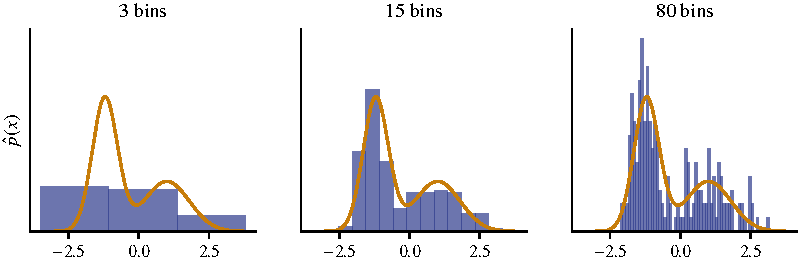
\includegraphics[width=0.85\linewidth]{figures/hist_density.pdf}
\caption{Histogram density estimates from the same 200 points with 3, 15 and 80 bins; the curve is the true density.}
\label{fig:histdens}
\end{figure}

\subsection{Bias and variance of the histogram density}\label{sec:biasvar}

The trade-off in Figure~\ref{fig:histdens} can be computed exactly. Work in one dimension with a bin
$C = [t_0, t_0 + h)$ that contains the point $x$, and let
\[
  p_C = P(X \in C) = \int_{t_0}^{t_0 + h} p(t)\, dt
\]
be the probability mass of the bin under the true density $p$.

\paragraph{Step 1: the count is binomial} Each of the $n$ independent training points falls in $C$ with probability
$p_C$, so $n_C = \sum_i \ind{X_i \in C}$ is a sum of $n$ independent Bernoulli variables:
\[
  n_C \sim \mathrm{Binomial}(n, p_C), \qquad \E[n_C] = n p_C, \qquad \Var[n_C] = n p_C (1 - p_C) .
\]

\paragraph{Step 2: mean and variance of the estimate} Since $\hat p(x) = n_C/(nh)$ is the count times a constant,
\[
  \E[\hat p(x)] = \frac{n p_C}{nh} = \frac{p_C}{h} = \frac{1}{h} \int_C p(t)\, dt,
  \qquad
  \Var[\hat p(x)] = \frac{n p_C (1 - p_C)}{(nh)^2} = \frac{p_C (1 - p_C)}{n h^2} .
\]
On average, the histogram returns the \emph{average of $p$ over the bin}, not $p(x)$.

\paragraph{Step 3: small bins} For small $h$, $p_C \approx h\, p(x)$ and $1 - p_C \approx 1$, so
\begin{equation}\label{eq:histvar}
  \Var[\hat p(x)] \approx \frac{h\, p(x)}{n h^2} = \frac{p(x)}{n h} .
\end{equation}
The variance falls with more data ($n$) and with wider bins ($h$): $nh\,p(x)$ is the expected count in the bin.

\paragraph{Step 4: the bias} Expand $p$ to first order around $x$, $p(t) \approx p(x) + p'(x)(t - x)$, and integrate
over the bin, whose centre is $t_0 + h/2$:
\[
  \E[\hat p(x)] = \frac{1}{h} \int_{t_0}^{t_0 + h} \big[p(x) + p'(x)(t - x)\big] dt
  = p(x) + p'(x) \Big(t_0 + \frac{h}{2} - x\Big) .
\]
The bias $\E[\hat p(x)] - p(x) = p'(x)\,(t_0 + h/2 - x)$ is proportional to the slope of the density and to the
distance from $x$ to the bin centre, which is at most $h/2$. The bias grows with the bin width.

\paragraph{Step 5: from one point to the whole line} For any estimator $\hat p$ of a number $p$, write
$\hat p - p = (\hat p - \E\hat p) + (\E\hat p - p)$ and expand the square; the cross term has zero mean because
$\E[\hat p - \E\hat p] = 0$, so
\[
  \E\big[(\hat p(x) - p(x))^2\big] = \big(\E[\hat p(x)] - p(x)\big)^2 + \Var[\hat p(x)]
  = \text{bias}^2 + \text{variance} .
\]
(Note~4, Section~6, meets the same decomposition for prediction errors.) Now integrate both terms over $x$.
\emph{Bias:} as $x$ moves across one bin, the offset $u = t_0 + h/2 - x$ runs uniformly over $[-h/2, h/2]$, and
$\int_{-h/2}^{h/2} u^2\, du = h^3/12$. Treating $p'$ as constant on the bin, with value $p'(x_C)$ at its centre $x_C$,
the integrated squared bias of one bin is $p'(x_C)^2\, h \cdot h^2/12$. Summing over the bins,
$\sum_C p'(x_C)^2\, h \approx \int p'(x)^2\, dx$, a Riemann sum. \emph{Variance:} integrating \eqref{eq:histvar} gives
$\int p(x)/(nh)\, dx = 1/(nh)$, because $\int p = 1$. Together they give the \emph{integrated mean squared error}
\begin{equation}\label{eq:imse}
  \mathrm{IMSE}(h) \approx \frac{h^2}{12} R(p') + \frac{1}{nh}, \qquad R(p') = \int p'(x)^2\, dx .
\end{equation}

\paragraph{Step 6: the best width} This is a function of one variable; set its derivative to zero:
\[
  \frac{d\,\mathrm{IMSE}}{dh} = \frac{h}{6} R(p') - \frac{1}{n h^2} = 0
  \quad\Longrightarrow\quad
  h^* = \Big(\frac{6}{n\, R(p')}\Big)^{1/3} \propto n^{-1/3} .
\]
At $h^*$ the squared bias is exactly half of the variance, and substituting back gives
$\mathrm{IMSE}(h^*) = \tfrac{3}{2}\,(nh^*)^{-1} \propto n^{-2/3}$. For a Gaussian of standard deviation $\sigma$,
$R(p') = 1/(4\sqrt{\pi}\,\sigma^3)$ and the formula becomes \emph{Scott's rule}
$h^* = (24\sqrt\pi)^{1/3}\, \sigma\, n^{-1/3} \approx 3.49\, \sigma\, n^{-1/3}$~\cite{scott1979}. Freedman and
Diaconis proposed the robust alternative $h = 2\,\mathrm{IQR}\cdot n^{-1/3}$, based on the interquartile range
IQR~\cite{freedman1981}, a good default in practice. (Inserting $\sigma = \mathrm{IQR}/1.349$ into Scott's rule would
give $2.59\,\mathrm{IQR}\cdot n^{-1/3}$; the smaller constant 2 errs towards narrower bins for non-Gaussian data.)

\begin{worked}{bias, variance and the best bin width}
Let $p$ be the standard normal density, $n = 100$, and estimate $p(1) = 0.2420$ with the bin $[1, 1 + h)$.
\begin{itemize}
\item $h = 0.5$: with the standard normal distribution function $\Phi$ from a table or a calculator
($\Phi(1) = 0.84134$, $\Phi(1.1) = 0.86433$, $\Phi(1.5) = 0.93319$), $p_C = \Phi(1.5) - \Phi(1) = 0.0918$, so $\E[\hat p(1)] = 0.0918/0.5 = 0.184$. The bias is
$0.184 - 0.242 = -0.058$ (Step~4 predicts $p'(1)\, h/2 = -0.242 \times 0.25 = -0.060$, since $p'(x) = -x\,p(x)$
for the standard normal, so $p'(1) = -0.242$). The standard deviation is
$\sqrt{0.0918 \times 0.9082/(100 \times 0.25)} = 0.058$. Mean squared error: $0.058^2 + 0.058^2 \approx 0.0067$.
\item $h = 0.1$: $p_C = \Phi(1.1) - \Phi(1) = 0.0230$, $\E[\hat p(1)] = 0.230$, bias $-0.012$; standard deviation
$\sqrt{0.0230 \times 0.9770/(100 \times 0.01)} = 0.150$. Mean squared error $\approx 0.0226$.
\end{itemize}
The narrow bin is almost unbiased but about 2.6 times noisier (standard deviation 0.150 against 0.058); with
$n = 100$ the wide bin wins. For $n = 1000$ points from
a standard normal, Scott's rule gives $h^* = 3.49 \times 1000^{-1/3} = 0.349$, about 18 bins over the range $[-3.2,
3.2]$ where the sample lies; Freedman--Diaconis (IQR $= 1.349$) gives $0.270$. With $n = 8000$ both widths halve.
\end{worked}

Figure~\ref{fig:biasvar} carries out the exact computation for the two-peaked density of Figure~\ref{fig:histdens}.
For $n = 200$ the error is smallest with about 19 bins, close to the 15 bins of the middle panel of
Figure~\ref{fig:histdens}; with $n = 2000$ the optimum moves to about 42 bins, a factor $2.2$, close to the predicted
$10^{1/3} = 2.15$.

\begin{figure}[h]
\centering
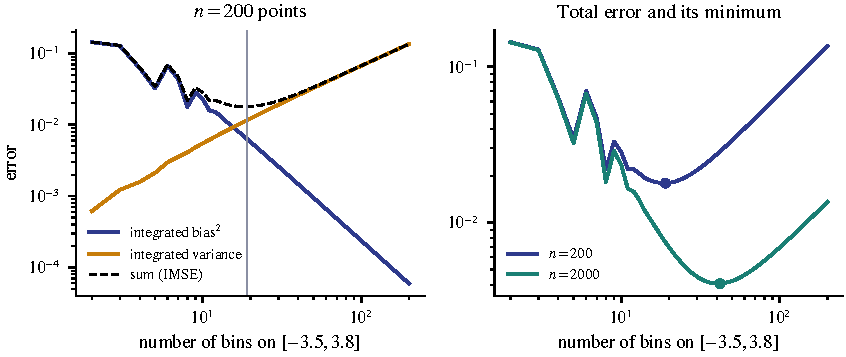
\includegraphics[width=0.9\linewidth]{figures/n3_biasvar.pdf}
\caption{Exact integrated squared bias and integrated variance of the histogram for the density of
Figure~\ref{fig:histdens}, as functions of the number of bins. Left: $n = 200$; the vertical line marks the minimum of
the sum (19 bins). Right: the total error for $n = 200$ and $n = 2000$. The wiggles at few bins come from where the
bin edges fall relative to the two peaks.}
\label{fig:biasvar}
\end{figure}

\paragraph{In $d$ dimensions} The cell has volume $h^d$, so the variance becomes $p(\x)/(nh^d)$, while the bias is
still of order $h$ (times the gradient of $p$). The integrated error has the form $A h^2 + B/(nh^d)$, with
$A \propto \int \norm{\nabla p}^2 d\x$ from the bias and $B = 1$ from $\int p = 1$ in the variance; only the powers of
$h$ and $n$ matter for the scaling. Minimising over $h$,
\[
  2Ah - \frac{d\,B}{n h^{d+1}} = 0 \quad\Longrightarrow\quad h^* = \Big(\frac{d\,B}{2A\,n}\Big)^{1/(d+2)} \propto n^{-1/(d+2)},
\]
and both terms then scale as $n^{-2/(d+2)}$~\cite{scott2015}. To halve the integrated mean squared error one needs $2^{(d+2)/2}$ times more
data: about $2^{3/2} \approx 2.8$ times more in $d = 1$ but $2^{6} = 64$ times more in $d = 10$. This is the curse of
dimensionality in its most quantitative form.

\begin{physics}{histograms are the language of experiments}
Most results in particle and nuclear physics are histograms: event counts in bins of an invariant mass, a momentum or
an angle. One of the channels of the 2012 Higgs-boson observation by ATLAS and CMS was a localised excess of events
near 125~GeV in the histogram of diphoton invariant masses~\cite{atlas2012,cms2012}. Many analyses use a
\emph{binned likelihood fit}, which treats each count as Poisson with a mean predicted by a
signal-plus-background model --- the density-estimation rule of Section~\ref{sec:hist}, turned into a statistical test. The
physicist's choice of binning is exactly the bias--variance compromise of Figure~\ref{fig:biasvar}: bins much wider
than the detector resolution wash out a narrow peak, bins much narrower leave a handful of events in each.
\end{physics}

\section{More features help --- up to a point}\label{sec:features}

Take the two-class problem of Note~1 (signal and background events described by two observables) with $n = 400$
training events and classify with histograms (Figure~\ref{fig:histclass}). Using only $x_1$ with 8 bins, the
classifier reaches 20.2\% test error. Adding $x_2$ with an $8 \times 8$ grid lowers it to 14.4\%: the second feature
carries information the first lacks. Refining to $40 \times 40$ cells lowers the \emph{training} error to 5.2\% but
raises the test error to 34.6\%. With 1600 cells and 400 points, most cells hold zero or one example; the
predictions in those cells are noise or a default. The same table of counts has gone from summarising the data to
memorising it.

\begin{figure}[h]
\centering
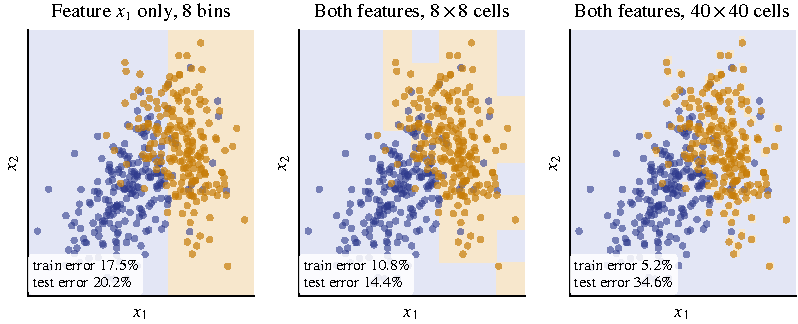
\includegraphics[width=0.9\linewidth]{figures/hist_classifier.pdf}
\caption{Histogram classifiers on 400 training events (indigo: background, amber: signal). Shaded regions show the
predicted class; empty cells predict the overall majority class. Errors are measured on the training set and on 4000
fresh test events.}
\label{fig:histclass}
\end{figure}

The numbers behind the figure make the mechanism visible. On the $8 \times 8$ grid, 46 of the 64 cells are occupied,
with on average 8.7 training points each: enough for a majority vote to mean something. On the $40 \times 40$ grid,
only 281 of the 1600 cells (18\%) are occupied, and 193 of those hold a single point. A single point decides the
prediction of its whole cell, and the empty cells --- 82\% of the grid --- all receive the fallback class. The
hand-worked example of Section~\ref{sec:formulas} showed the same effect on ten points.

Two lessons follow. First, the number of cells is the knob that sets the \emph{capacity} of the histogram ---
how many different functions it can represent. A two-class histogram with $M$ cells can label each cell 0 or 1
independently, so it represents $2^M$ different classifiers: $2^9 = 512$ for the $3 \times 3$ grid of the worked
example, $2^{100} \approx 1.3 \times 10^{30}$ for $m = 10$ bins on $d = 2$ axes, and $2^{10^{10}}$ for $m = 10$ and
$d = 10$. The capacity must be chosen on data not used for counting; Note~4, Section~5, treats capacity, underfitting
and overfitting in general. Second, the knob runs out of room quickly: every additional feature multiplies the number
of cells by $m$, and the number of representable functions grows even faster, while the amount of data stays the
same.

\section{The curse of dimensionality}\label{sec:curse}

The phrase is Bellman's, from his work on dynamic programming, where tabulating a function of many state variables
on a grid becomes impossible~\cite{bellman1957,bellman1961}. For
learning it has four faces, each of which can be computed with elementary probability and geometry. Throughout this
section the data are uniform in the unit cube $[0, 1]^d$; real data are not, and Section~\ref{sec:escape} returns to
what that changes.

\subsection{Cells outnumber data}\label{sec:cells}

Even a very coarse grid explodes. Cut each axis into only $m = 4$ bins (its quartiles) and take a million uniform
points. In $d = 1$ each of the 4 cells holds $250\,000$ points; in $d = 5$ there are $4^5 = 1024$ cells with about 980
points each. In $d = 10$ there are $4^{10} \approx 1.05 \times 10^6$ cells, about one point per cell, and 39\% of the
cells are empty. In $d = 20$ there are $1.1 \times 10^{12}$ cells and at most one in a million is occupied: a new test
point almost surely lands in a cell the training data never visited. Figure~\ref{fig:curse} (left) shows the same
collapse with $n = 10^5$ points and $m = 10$ bins per axis: on average $10^4$, $10^3$ and $10^2$ points per cell for
$d = 1, 2, 3$, but $10^{-5}$ for $d = 10$ and $10^{-95}$ for $d = 100$. A $28 \times 28$ grey-scale image has
$d = 784$, and $10^{784}$ dwarfs the roughly $10^{80}$ atoms in the observable universe.

\paragraph{Expected occupancy} With $M = m^d$ cells of equal probability, each training point lands in a given cell
$C$ with probability $1/M$, independently of the others. Hence $n_C \sim \mathrm{Binomial}(n, 1/M)$ and
\[
  \E[n_C] = \frac{n}{M} = \frac{n}{m^d} .
\]
To have on average $\nu$ points per cell we need $n = \nu\, m^d$ examples: exponential in $d$.

\paragraph{Probability that a cell is empty} All $n$ points must miss the cell:
\[
  P(n_C = 0) = \Big(1 - \frac{1}{M}\Big)^n = \exp\Big(n \log\Big(1 - \frac{1}{M}\Big)\Big) \approx e^{-n/M},
\]
using $\log(1 - u) \approx -u$ for small $u = 1/M$. The expected number of occupied cells follows by linearity
of expectation: it is the sum over the $M$ cells of the probability that the cell is occupied,
\[
  \E[\#\text{occupied cells}] = \sum_C P(n_C \ge 1) = M \Big(1 - \Big(1 - \frac{1}{M}\Big)^n\Big),
\]
and it can never exceed $n$.

\paragraph{Probability that a test point lands in an empty cell} A uniform test point falls in cell $C$ with
probability $1/M$, independently of the training set. Summing over the cells,
\[
  P(\text{test cell empty}) = \sum_C P(\text{test in } C)\, P(n_C = 0) = M \cdot \frac{1}{M} \Big(1 - \frac{1}{M}\Big)^n
  = \Big(1 - \frac{1}{M}\Big)^n \approx e^{-n/m^d} .
\]
For a non-uniform distribution with cell probabilities $p_C$ the same argument gives
$\sum_C p_C (1 - p_C)^n$.

\begin{worked}{how many events does a binned analysis need}
An experiment records $n = 10^6$ events and bins each observable into $m = 20$ bins. Assuming (optimistically)
uniform occupancy:

\begin{center}\small
\begin{tabular}{@{}ccccc@{}}\toprule
$d$ & cells $20^d$ & points per cell $n/20^d$ & $P(\text{test cell empty}) \approx e^{-n/20^d}$ & $n$ for 10 per cell \\ \midrule
1 & 20 & 50\,000 & $\approx 0$ & 200 \\
2 & 400 & 2500 & $\approx 0$ & 4000 \\
3 & 8000 & 125 & $\approx 5 \times 10^{-55}$ & $8 \times 10^{4}$ \\
4 & $1.6 \times 10^5$ & 6.25 & 0.0019 & $1.6 \times 10^{6}$ \\
5 & $3.2 \times 10^6$ & 0.31 & 0.73 & $3.2 \times 10^{7}$ \\
6 & $6.4 \times 10^7$ & 0.016 & 0.98 & $6.4 \times 10^{8}$ \\ \bottomrule
\end{tabular}
\end{center}
A million events support a four-dimensional histogram at most; with five observables, three test events in four land in
an empty cell, and ten events per cell would need 32 million events.
\end{worked}

\subsection{Neighbourhoods stop being local}\label{sec:edge}

To capture a fraction $\rho$ of uniformly distributed data in the unit cube we can use a sub-cube of edge $e$. The
fraction of the data it contains equals its volume, so
\[
  e^d = \rho \quad\Longrightarrow\quad e = \rho^{1/d} = \exp\Big(\frac{\ln \rho}{d}\Big) \xrightarrow[d \to \infty]{} 1 .
\]
Read in the other direction: a sub-cube that spans half of every coordinate, $e = 1/2$, contains a fraction $2^{-d}$
of the data --- one point in a thousand when $d = 10$ and one in a million when $d = 20$.

\begin{worked}{edge length of a neighbourhood}
\begin{center}\small
\begin{tabular}{@{}lccccc@{}}\toprule
 & $d = 1$ & $d = 2$ & $d = 3$ & $d = 10$ & $d = 100$ \\ \midrule
edge to capture $\rho = 1\%$ of the data & 0.01 & 0.10 & 0.22 & 0.63 & 0.95 \\
edge to capture $\rho = 10\%$ of the data & 0.10 & 0.32 & 0.46 & 0.79 & 0.98 \\ \bottomrule
\end{tabular}
\end{center}
For example, $0.01^{1/10} = 10^{-0.2} = 0.63$. A ``neighbourhood'' that contains enough points to average over spans
almost the whole range of every coordinate.
\end{worked}

\subsection{Volume lives near the boundary}\label{sec:shell}

The volume of a ball of radius $r$ in $d$ dimensions is $V_d\, r^d$, with
$V_d = \pi^{d/2} / \Gamma(d/2 + 1)$ the volume of the unit ball ($V_1 = 2$, $V_2 = \pi$, $V_3 = 4\pi/3$). The Gamma
function extends the factorial: $\Gamma(k + 1) = k!$ for integer $k$, so for even $d$ simply
$V_d = \pi^{d/2}/(d/2)!$; for odd $d$ one also needs $\Gamma(1/2) = \sqrt\pi$ and $\Gamma(z + 1) = z\,\Gamma(z)$. The shell of
points within a fraction $\varepsilon$ of the surface of the unit ball therefore holds the fraction
\[
  \frac{V_d - V_d (1 - \varepsilon)^d}{V_d} = 1 - (1 - \varepsilon)^d
\]
of the volume, which tends to one for any fixed $\varepsilon > 0$. Similarly, the ball of radius 1 inscribed in the
cube $[-1, 1]^d$ (volume $2^d$) occupies the fraction $V_d / 2^d$, while the corners of the cube are at distance
$\sqrt d$ from the centre.

\begin{worked}{the shell, the ball and the cube}
\begin{center}\small
\begin{tabular}{@{}lccccccc@{}}\toprule
$d$ & 1 & 2 & 3 & 5 & 10 & 20 & 50 \\ \midrule
outer 10\% shell, $1 - 0.9^d$ & 0.10 & 0.19 & 0.27 & 0.41 & 0.65 & 0.88 & 0.995 \\
inscribed ball / cube, $V_d / 2^d$ & 1 & 0.785 & 0.524 & 0.164 & 0.0025 & $2.5 \times 10^{-8}$ & $1.5 \times 10^{-28}$ \\
distance of a corner, $\sqrt d$ & 1 & 1.41 & 1.73 & 2.24 & 3.16 & 4.47 & 7.07 \\ \bottomrule
\end{tabular}
\end{center}
For instance, $V_{10} = \pi^5/5! = 306.0/120 = 2.550$ and $2.550/1024 = 0.0025$. In $d = 10$ only one point in 400
of the cube lies inside its inscribed ball; almost all of the cube is in its corners.
\end{worked}

The same geometry explains where a standard Gaussian $\vect{z} \sim \Normal(\vect{0}, I_d)$ puts its samples.
Note~2, Question~C4, shows that $\E\norm{\vect{z}}^2 = d$ and $\Var\norm{\vect{z}}^2 = 2d$, so
$\norm{\vect{z}}^2 \approx d \pm \sqrt{2d}$. The fluctuation $\sqrt{2d}$ belongs to the \emph{squared} radius; by the
same first-order expansion of the square root used in Section~\ref{sec:concentrate} below, the radius itself is
$\norm{\vect{z}} \approx \sqrt d \pm \sqrt{2d}/(2\sqrt d) = \sqrt d \pm 0.71$: a thin shell, whose width does not
grow with $d$ (in $d = 50$ the radius has mean $7.04$ and standard deviation $0.71$). The typical samples are nowhere near the most
probable point, the origin. Why the shell wins: the probability of the thin shell between radii $r$ and $r + dr$ is
(density) $\times$ (shell volume) $\propto e^{-r^2/2} \cdot r^{d-1} dr$, because the surface of a sphere of radius $r$
grows like $r^{d-1}$. Its logarithm $(d - 1) \ln r - r^2/2$ has derivative $(d - 1)/r - r$, which vanishes at
$r = \sqrt{d - 1}$. The density at the centre is the highest, but there is almost no volume there.

\subsection{Distances concentrate}\label{sec:concentrate}

Take a query point and many data points whose coordinates are independent and identically distributed (such as
uniform data in the cube), and let $\mathrm{dist}_{\max}$ and $\mathrm{dist}_{\min}$ be the distances from the query
to the farthest and to the nearest data point. As $d$ grows, the \emph{relative contrast}
$(\mathrm{dist}_{\max} - \mathrm{dist}_{\min})/\mathrm{dist}_{\min}$ tends to zero in probability, that is
$\mathrm{dist}_{\max}/\mathrm{dist}_{\min} \to 1$ (Figure~\ref{fig:curse}, right): the nearest neighbour is hardly
nearer than the farthest~\cite{beyer1999}. Data of low intrinsic dimension escape this (Section~\ref{sec:escape}).
Any method that relies on ``nearby'' points --- histograms, and also the neighbourhood methods of Note~5 --- loses its
footing. A short computation shows why.

\paragraph{One coordinate} Let $U, V$ be independent and uniform on $[0, 1]$, so that $\E[U^k] = \int_0^1 u^k\, du =
1/(k + 1)$: $\E[U] = 1/2$, $\E[U^2] = 1/3$, $\E[U^3] = 1/4$, $\E[U^4] = 1/5$. For the difference $\Delta_1 = U - V$,
\[
  \E[\Delta_1^2] = \E[U^2] - 2\,\E[U]\,\E[V] + \E[V^2] = \tfrac13 - \tfrac12 + \tfrac13 = \tfrac16 .
\]
For the variance of $\Delta_1^2$ we need the fourth moment. Expanding $(U - V)^4$ with the binomial coefficients
$1, 4, 6, 4, 1$ and using independence,
\[
  \E[\Delta_1^4] = \E[U^4] - 4\,\E[U^3]\,\E[V] + 6\,\E[U^2]\,\E[V^2] - 4\,\E[U]\,\E[V^3] + \E[V^4]
  = \tfrac15 - \tfrac12 + \tfrac23 - \tfrac12 + \tfrac15 = \tfrac{1}{15},
\]
so $\Var[\Delta_1^2] = \E[\Delta_1^4] - (\E[\Delta_1^2])^2 = \tfrac{1}{15} - \tfrac{1}{36} = \tfrac{7}{180}$.

\paragraph{All coordinates} The squared distance between two uniform points of $[0, 1]^d$ is
$\Delta^2 = \sum_{j=1}^d (U_j - V_j)^2$, a sum of $d$ independent terms, each distributed like $\Delta_1^2$. Means and
variances add:
\[
  \E[\Delta^2] = \frac{d}{6}, \qquad \Var[\Delta^2] = \frac{7d}{180}, \qquad
  \frac{\sqrt{\Var[\Delta^2]}}{\E[\Delta^2]} = \frac{\sqrt{7d/180}}{d/6} = \frac{1.18}{\sqrt d} .
\]
The typical squared distance grows like $d$, its spread only like $\sqrt d$, so the \emph{relative} spread shrinks like
$1/\sqrt d$. All pairwise distances become nearly equal to $\sqrt{d/6}$.

\paragraph{From squared distance to distance} Because $\Delta^2$ fluctuates little around its mean, expand the square
root to first order (a Taylor expansion, $\sqrt{a + \epsilon} \approx \sqrt a + \epsilon/(2\sqrt a)$, with
$a = \E[\Delta^2]$): $\Delta \approx \sqrt{\E[\Delta^2]} + (\Delta^2 - \E[\Delta^2])/(2\sqrt{\E[\Delta^2]})$. Hence
\[
  \mathrm{sd}(\Delta) \approx \frac{\mathrm{sd}(\Delta^2)}{2\sqrt{\E[\Delta^2]}} = \frac{\sqrt{7d/180}}{2\sqrt{d/6}}
  = \frac12\sqrt{\frac{7}{30}} \approx 0.24,
  \qquad
  \frac{\mathrm{sd}(\Delta)}{\sqrt{\E[\Delta^2]}} \approx \frac{0.24}{\sqrt{d/6}} = \frac{0.59}{\sqrt d} .
\]
The factors $\sqrt d$ cancel: the spread of the distance itself does not depend on $d$ at all, while its mean grows
like $\sqrt d$, so its relative spread is half that of $\Delta^2$.

\begin{worked}{distances between random points}
\begin{center}\small
\begin{tabular}{@{}lcccc@{}}\toprule
$d$ & 2 & 10 & 100 & 1000 \\ \midrule
$\E[\Delta^2] = d/6$ & 0.333 & 1.667 & 16.67 & 166.7 \\
standard deviation of $\Delta^2$, $\sqrt{7d/180}$ & 0.279 & 0.624 & 1.97 & 6.24 \\
mean distance $\Delta$ (simulated) & 0.52 & 1.27 & 4.07 & 12.91 \\
standard deviation of the distance (simulated) & 0.25 & 0.24 & 0.24 & 0.24 \\
relative spread of the distance & 0.47 & 0.19 & 0.059 & 0.019 \\ \bottomrule
\end{tabular}
\end{center}
(The simulated rows use $20\,000$ random pairs.) They confirm the expansion above: the spread of the distance stays
near $0.24$, and from $d = 10$ on the last row matches $0.59/\sqrt d$. The mean grows like
$\sqrt{d/6}$: in $d = 1000$ almost every pair of points is at distance $12.9 \pm 0.24$, so ``near'' and ``far'' differ
by a few per cent.
\end{worked}

\begin{figure}[h]
\centering
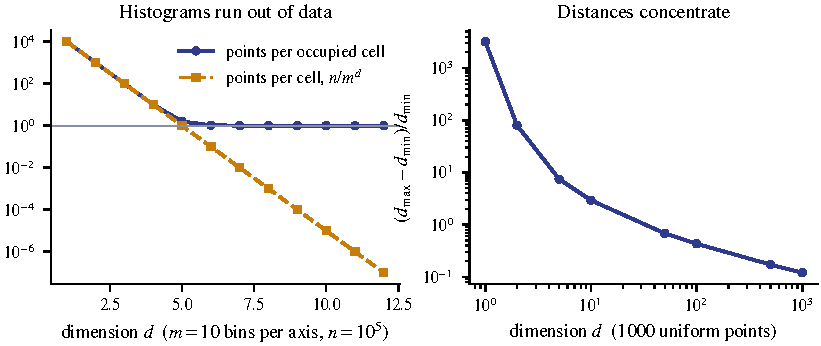
\includegraphics[width=0.85\linewidth]{figures/curse.pdf}
\caption{Left: average number of points per cell and per \emph{occupied} cell for $n = 10^5$ uniform points and 10
bins per axis. Beyond $d \approx 5$ occupied cells hold a single point and almost all cells are empty. Right: the
relative contrast $(\mathrm{dist}_{\max} - \mathrm{dist}_{\min})/\mathrm{dist}_{\min}$ of the distances from a random
query to 1000 uniform points (median of 20 trials); in the axis label, $d_{\max}$ and $d_{\min}$ stand for these
distances, not for dimensions.}
\label{fig:curse}
\end{figure}

\begin{keyidea}[The curse]
A method that needs examples \emph{near} every query point needs a number of examples that grows exponentially with
the dimension, because the number of cells to be filled does. A fixed grid stays useful only while $n$ is much larger
than $m^d$, which for realistic samples means two to four dimensions. The number of functions the grid can represent
grows faster still: with $M = m^d$ cells and two classes there are $2^M$ possible classifiers, and $n$ examples fix the
labels of at most $n$ of the $M$ cells --- the rest are left to the fallback rule. Every method pays some price in high
dimension; methods that exploit structure (Section~\ref{sec:escape}) pay far less.
\end{keyidea}

\section{Why learning in high dimension is possible at all}\label{sec:escape}

Image classifiers work on inputs with $d \approx 10^5$; language models on sequences of thousands of tokens. They do
not contradict the curse; they exploit structure that uniform random data do not have.

\begin{enumerate}
\item \textbf{Low intrinsic dimension.} Real data occupy a tiny, structured part of $\R^d$. Natural images of a given
size are a vanishing subset of all pixel arrays, plausibly close to a manifold of much lower dimension. Estimates
of the intrinsic dimension of standard image datasets range from about 10 (MNIST) to a few tens (ImageNet), against
input dimensions from several hundred to more than $10^5$, and learning is easier when the intrinsic dimension is
lower~\cite{pope2021}.
\item \textbf{Smoothness and invariance.} The target changes slowly or not at all along many directions: a
translated cat is still a cat. Architectures that build these invariances in (convolutions for translations,
graph networks for permutations, equivariant networks for rotations) reduce the effective number of functions to be
distinguished.
\item \textbf{Adaptive partitions.} Instead of a fixed grid, split only where the data require it and only along
informative directions. A decision tree does exactly this; its number of cells grows with $n$, not with $m^d$.
\item \textbf{Learned representations.} Map the input to a lower-dimensional space in which simple methods work,
and learn the map from data. The embeddings of Note~1, Section~3, are such maps.
\end{enumerate}

\subsection{Decision trees: adaptive histograms}\label{sec:trees}

A \emph{decision tree} builds its cells one cut at a time. Starting from the whole box, it chooses one feature $j$
and one threshold $\tau$ and splits the data into $x_j < \tau$ and $x_j \ge \tau$; then it splits each half again, and so on.
The leaves are boxes, exactly like histogram cells, and each leaf predicts by majority vote (or by the mean of $y$
for regression). The difference is that the cuts are \emph{chosen by the data}: where the classes are already
separated the tree stops, and features that carry no information are never used.

\paragraph{How to choose a cut} A cut is good if its two halves are purer than the parent. A standard measure of
impurity of a set $S$ of training points with class frequencies $\hat\pi_1, \dots, \hat\pi_K$ is the \emph{Gini impurity}
\[
  G(S) = \sum_{k=1}^K \hat\pi_k (1 - \hat\pi_k) = 1 - \sum_{k=1}^K \hat\pi_k^2 ,
\]
which is zero for a pure set and equals $2\hat\pi_1(1 - \hat\pi_1)$ for two classes. A cut of $S$ into $L$ and $R$ is scored by
the size-weighted impurity of the children, $(|L|\, G(L) + |R|\, G(R))/|S|$, and the tree takes the cut with the lowest
score~\cite{breiman1984}. For regression the impurity is the variance of $y$ in the set, so the best cut is the one
that most reduces the sum of squared errors around the leaf means. On the eight calibration points of the regression
example above, for instance, the sum of squared errors around the overall mean is $19.12$; the best single cut,
$x < 2.45$ (midway between 1.8 and 3.1), lowers it to $1.612 + 0.180 = 1.792$, and the two leaves predict $1.86$ and
$4.9$ --- the bins of width 2 found again, now chosen by the data.

\begin{worked}{the first cut of a tree}
Return to the ten points of Table~\ref{tab:toy}. The root has $\hat\pi_1 = 4/10$, so $G = 2 \times 0.4 \times 0.6 =
0.48$. Restrict the candidate thresholds to the grid lines $\tau = 1$ and $\tau = 2$ of the histogram:

\begin{center}\small
\begin{tabular}{@{}lccccc@{}}\toprule
cut & left $(N_0, N_1)$ & right $(N_0, N_1)$ & $G(L)$ & $G(R)$ & weighted Gini \\ \midrule
$x_1 < 1$ & $(2, 0)$ & $(4, 4)$ & 0 & 0.50 & $(2 \cdot 0 + 8 \cdot 0.5)/10 = 0.40$ \\
$x_1 < 2$ & $(4, 1)$ & $(2, 3)$ & 0.32 & 0.48 & $(5 \cdot 0.32 + 5 \cdot 0.48)/10 = 0.40$ \\
$x_2 < 1$ & $(2, 0)$ & $(4, 4)$ & 0 & 0.50 & $0.40$ \\
$x_2 < 2$ & $(5, 0)$ & $(1, 4)$ & 0 & 0.32 & $(5 \cdot 0 + 5 \cdot 0.32)/10 = 0.16$ \\ \bottomrule
\end{tabular}
\end{center}
The cut $x_2 < 2$ wins clearly. Its left leaf is pure (class 0) and its right leaf predicts class 1 with
$\hat P(Y = 1) = 4/5$; only \toy{10} is misclassified, the same training error as the nine-cell histogram, but with two cells
and none empty (Figure~\ref{fig:toy}, right). The query $q_1 = (2.5, 1.5)$, which fell in an empty histogram cell,
is now predicted from five points (class 0), and $q_2$ and $q_3$ from five points (class 1). Among the grid cuts,
splitting the right leaf again at $x_1 < 2$ would lower its weighted Gini only from 0.32 to 0.30; a stopping rule such
as ``at least three points per leaf'' ends the growth here. Counting training errors instead of Gini would choose the
same cut (1 error against 3 or 4 for the others).

\textbf{Without the grid.} Algorithm~\ref{alg:tree} does not stop at the grid lines: it tries every threshold between
consecutive values. On these data it finds $x_2 < 2.2$, midway between \toy{10} ($x_2 = 2.1$) and the lowest class-1
values (\toy{7} and \toy{9}, $x_2 = 2.3$). That cut gives the pure leaves $(6, 0)$ and $(0, 4)$, weighted Gini 0 and no training error.
With only ten points such a perfect split is as much luck as signal --- a first sign of the variance of trees grown
until their leaves are pure. We kept the grid thresholds only to compare the tree with the histogram.
\end{worked}

\begin{algorithm}[htbp]
\caption{Growing a classification tree greedily (CART); comments give the regression variant}
\label{alg:tree}
\small
\begin{algorithmic}[1]
\Require training set $S$; hyperparameters: maximum depth $D_{\max}$, minimum leaf size $n_{\min}$
\Function{Grow}{$S$, depth}
  \If{depth $= D_{\max}$ \textbf{or} $|S| < 2 n_{\min}$ \textbf{or} all labels in $S$ are equal}
    \State \Return \Call{Leaf}{class frequencies of $S$} \Comment{regression: the mean of $y$ in $S$}
  \EndIf
  \State best $\gets (\infty, \text{none}, \text{none})$
  \For{$j = 1, \dots, d$}
    \State sort $S$ by $x_j$ \Comment{$O(|S| \log |S|)$}
    \For{each threshold $\tau$ between consecutive distinct values of $x_j$}
      \State $L \gets \{i \in S : x_{ij} < \tau\}$, $R \gets S \setminus L$; \ $g \gets (|L| G(L) + |R| G(R))/|S|$ \Comment{counts updated incrementally}
      \Statex \hspace{3.2em}\Comment{regression: replace $G$ by the variance of $y$}
      \If{$|L|, |R| \ge n_{\min}$ \textbf{and} $g <$ best score} best $\gets (g, j, \tau)$ \EndIf
    \EndFor
  \EndFor
  \If{no admissible cut was found} \Return \Call{Leaf}{class frequencies of $S$} \EndIf
  \State split $S$ into $L$ and $R$ with the best $(j, \tau)$
  \State $T_L \gets{}$\Call{Grow}{$L$, depth$+1$}; \ $T_R \gets{}$\Call{Grow}{$R$, depth$+1$}
  \State \Return \Call{Node}{$j, \tau, T_L, T_R$}
\EndFunction
\Function{Predict}{tree, $\x$}
  \While{the current node is not a leaf}
    \State go to the left child if $x_j < \tau$, otherwise to the right child
  \EndWhile
  \State \Return the majority class (regression: the mean) stored in the leaf
\EndFunction
\end{algorithmic}
\end{algorithm}

\begin{runtime}{decision tree (Algorithm~\ref{alg:tree})}
Symbols: $n$ points, $d$ features, $K$ classes, depth $D$.
\begin{itemize}[leftmargin=1.2em]
\item \textbf{Training:} at one node with $n_S$ points, each feature costs a sort, $O(n_S \log n_S)$, plus a sweep over
the thresholds that updates the class counts of $L$ and $R$ one point at a time, $O(n_S K)$. The nodes of one level
partition the data, so a level costs $O(d\, n (\log n + K))$ and the whole tree $O(D\, d\, n(\log n + K))$.
Pre-sorting once, or binning each feature into a few hundred values as LightGBM does, removes the $\log n$.
For a regression tree, running sums of $y$ and $y^2$ in $L$ and $R$ replace the $K$ class counts (the variance is
$\overline{y^2} - \bar y^2$), so the sweep costs $O(n_S)$ instead of $O(n_S K)$.
\item \textbf{Prediction per query:} $O(D)$ comparisons --- one per level --- independent of $d$ and $n$.
\item \textbf{Memory:} $O(\text{number of nodes}) \le O(\min(2^{D}, n))$, since every leaf holds at least one point.
\item \textbf{In practice:} with $n = 10^6$, $d = 100$ and depth 10, the bound is about
$10 \times 100 \times 10^6 \times 20 = 2 \times 10^{10}$ elementary operations (taking $\log_2 n \approx 20$), of order
a minute in compiled code. Binned implementations drop the factor $\log n$ and finish in seconds; GPUs help mainly when
hundreds of trees are grown for an ensemble.
\end{itemize}
Unlike the grid, nothing here is exponential in $d$: the tree pays for a feature only when it uses it.
\end{runtime}

A single deep tree has the same weakness as a fine histogram --- leaves with one or two points, high variance --- and
its depth must be chosen on held-out data (Note~4). Averaging many trees fixes this, as the box below explains.

\begin{physics}{many degrees of freedom, few that matter}
A configuration of the two-dimensional Ising model on a $40 \times 40$ lattice is a point in a space of $2^{1600}$
states, yet near the phase transition its physics is governed by one order parameter. Applying principal component
analysis to Monte Carlo configurations recovers the magnetisation as the leading direction without being told about
it, and locates the critical temperature~\cite{wang2016}. Statistical mechanics is, in this sense, a theory of low
intrinsic dimension; machine learning tries to discover such coordinates when no theory supplies them.
\end{physics}

\begin{modern}{the histogram's descendants}
Decision trees are adaptive histograms, and ensembles of them --- random forests and gradient-boosted trees --- are
still among the strongest and most widely used methods on tabular data of moderate size; in a 2022 benchmark they
often beat deep networks~\cite{grinsztajn2022}, although pretrained tabular models now compete with them on small
datasets~\cite{hollmann2025}. Boosted decision trees, introduced to particle physics around 2005~\cite{roe2005},
became one of the most widely used multivariate classifiers in the field for the following decade. Modern implementations even keep the literal histogram: LightGBM bins each feature into at most a
few hundred values and finds splits by scanning those per-feature histograms, which is what makes training on
millions of rows fast~\cite{ke2017}. Binning one feature at a time is cheap; binning all features jointly is what
the curse forbids.
\end{modern}

\section{From idea to algorithm}\label{sec:design}

Designing a learning algorithm follows a sequence that is worth making explicit once:
\begin{enumerate}
\item explain the idea in words (``count labels per cell, predict the majority'');
\item formalise it mathematically (the table and formulas of Section~\ref{sec:hist});
\item write pseudocode (Algorithm~\ref{alg:hist}), identifying its \emph{hyperparameters} --- quantities fixed before
training, here the bins --- and its \emph{parameters} --- quantities computed from data, here the counts;
\item implement, and test first on a small problem whose correct answer is known --- the ten points of
Table~\ref{tab:toy}, where every count can be checked by hand, or a 2-D synthetic set as in
Figure~\ref{fig:histclass} --- before running on real data;
\item analyse cost in time and memory;
\item evaluate on real data against other algorithms, with the methodology of Note~4.
\end{enumerate}
Step~5 deserves a closer look for histograms, because it shows the difference between a computational and a
statistical bottleneck.

\subsection{Cost analysis and the sparse variant}\label{sec:cost}

The dense arrays of Algorithms~\ref{alg:hist} and~\ref{alg:histreg} reserve a counter for every one of the $m^d$ cells,
although at most $n$ of them can ever be occupied. Storing only the occupied cells in a hash table (a Python
dictionary keyed by the tuple of bin indices) removes the exponential memory (Algorithm~\ref{alg:sparse}).

\begin{algorithm}[htbp]
\caption{Sparse histogram classifier: a hash table of occupied cells}
\label{alg:sparse}
\small
\begin{algorithmic}[1]
\Require as in Algorithm~\ref{alg:hist}
\Function{Train}{$\Dtrain$}
  \State $H \gets$ empty hash table \Comment{key: cell tuple $(c_1, \dots, c_d)$; value: vector of $K$ counts}
  \For{each $(\x_i, y_i) \in \Dtrain$}
    \State $c \gets \Call{CellIndex}{\x_i}$
    \If{$c \notin H$} \State $H[c] \gets (0, \dots, 0)$ \Comment{create the cell on first visit} \EndIf
    \State $H[c][y_i] \gets H[c][y_i] + 1$
  \EndFor
  \State $k_0 \gets$ the most frequent class in $\Dtrain$
\EndFunction
\Function{Predict}{$\x$}
  \State $c \gets \Call{CellIndex}{\x}$
  \If{$c \notin H$} \Return $k_0$ \Comment{empty cell} \EndIf
  \State \Return $\argmax_k H[c][k]$
\EndFunction
\end{algorithmic}
\end{algorithm}


\begin{runtime}{sparse histogram (Algorithm~\ref{alg:sparse})}
\begin{itemize}[leftmargin=1.2em]
\item \textbf{Training:} $O(nd)$ on average: hashing a key of $d$ integers costs $O(d)$, and a lookup or insertion
then costs $O(1)$ on average. No $O(Km^d)$ initialisation is needed.
\item \textbf{Prediction per query:} $O(d + K)$ on average, as for the dense array.
\item \textbf{Memory:} $O(M_{\mathrm{occ}}(d + K))$ with $M_{\mathrm{occ}} \le \min(n, m^d)$ occupied cells, each storing
its key ($d$ integers) and $K$ counts --- against $O(Km^d)$ for the dense array. Algorithm~\ref{alg:histreg} has the
same sparse version.
\end{itemize}
\end{runtime}

\begin{worked}{dense or sparse}
\textbf{By hand.} For the ten points of Table~\ref{tab:toy} with unit cells, Algorithm~\ref{alg:sparse} creates six
keys $(c_1, c_2)$ with their counts $(N_0, N_1)$:
\[
  \begin{gathered}
  (0,1) \mapsto (2,0), \qquad (1,0) \mapsto (1,0), \qquad (1,1) \mapsto (1,0), \\
  (2,0) \mapsto (1,0), \qquad (1,2) \mapsto (0,1), \qquad (2,2) \mapsto (1,3),
  \end{gathered}
\]
that is 12 counts instead of the $9 \times 2 = 18$ of the dense array, and $k_0 = 0$. The query $q_1 = (2.5, 1.5)$ has
the key $(2, 1)$, which is not in the table, so \textsc{Predict} returns $k_0 = 0$, as in the worked example of
Section~\ref{sec:formulas}.

\textbf{At scale.} Return to the binned analysis of Section~\ref{sec:cells}: $m = 20$ bins per axis and $n = 10^6$ events, now with
$d = 8$ observables and $K = 3$ classes. The dense array needs $3 \times 20^8 = 7.7 \times 10^{10}$ counters; at
4 bytes each, about 300~GB. The hash table holds at most $10^6$ cells, each with $8 + 3$ integers of 8 bytes: about
$10^6 \times 11 \times 8 \approx 90$~MB (a Python dictionary adds a small constant factor). A dense implementation
also flattens the tuple into one integer $c_1 + m c_2 + \dots + m^{d-1} c_d$; this number overflows a 64-bit integer
once $m^d > 2^{63} \approx 9.2 \times 10^{18}$, that is from $d = 15$ when $m = 20$. Tuples used as hash keys avoid
the problem.
\end{worked}

Training and prediction are as fast as any algorithm can be: one pass over the data for training, and $O(d + K)$
work per query that does not grow with $n$. The hash table removes the exponential memory, but it does not remove the
curse: by Section~\ref{sec:cells}, a query in the example above lands in an empty cell with probability
$e^{-10^6/20^8} \approx 0.99996$, and the classifier answers with the fallback class almost every time. The bottleneck is statistical, not computational.

\begin{keyidea}[Summary]
Partitioning the input space and counting gives a classifier (majority vote per cell), a regressor (mean per cell,
the minimiser of squared error) and a density estimator ($n_C/(n\,\mathrm{vol})$) in a few lines; training costs
$O(nd)$ plus one counter per cell and prediction $O(d)$ ($O(d + K)$ for the classifier). The histogram density has bias of order $h$ and variance
$p(x)/(nh)$; their balance gives $h^* \propto n^{-1/3}$ in one dimension and an error rate $n^{-2/(d+2)}$ in $d$
dimensions. The number of cells grows as $m^d$, so in high dimension cells are empty ($P \approx e^{-n/m^d}$),
neighbourhoods are not local (edge $\rho^{1/d}$), volume sits near the boundary ($1 - (1 - \varepsilon)^d$) and
distances concentrate (relative spread $\propto 1/\sqrt d$). Learning in high dimension succeeds by exploiting
structure --- low intrinsic dimension, smoothness, invariances --- through adaptive partitions such as decision trees
and learned representations.
\end{keyidea}

\begin{questions}
\begin{conceptual}
\item A classifier is asked about points where no training example lies. Explain how a histogram
classifier answers such a query, what it does when the query falls in an empty cell, and name two possible fallback rules with
one drawback of each.
\item For the histogram classifier, list the hyperparameters and the parameters. Which of them are computed from the
training data, and which must be fixed before counting?
\item Explain why the majority vote minimises the number of training errors inside a cell, and why the cell mean is
the best constant prediction under squared error.
\item Describe what happens to a histogram density estimate when the number of bins is very small and when it is very
large. Use the words bias and variance, say which choice gives the higher log-likelihood on the training data, and
explain why that does not make it the better choice.
\item True or false, with a justification: ``Adding a feature to a histogram classifier can never increase its test
error, because the new feature can only add information.''
\item A colleague proposes to choose the number of bins of a density histogram by maximising the log-likelihood of the
training data. What would this procedure choose, and why? Propose a way to choose the number of bins using only the
data, without a formula. (Hint: keep part of the data aside and evaluate the log-likelihood on it; compare
Question~D3.)
\item The count in a bin with expected value 4 fluctuates by about 50\%, a bin with expected value 400 by about 5\%.
Explain where these numbers come from and what they imply for choosing the bin width.
\item Why does the optimal bin width shrink as the number of data points grows? Why does it shrink only like
$n^{-1/3}$ and not like $1/n$?
\item In $d = 100$, a cube that contains 1\% of uniformly distributed data has an edge of 0.95. Explain what this
means for a method that averages over the ``neighbours'' of a query point.
\item What does it mean that ``distances concentrate'' in high dimension? Why is this harmful for any method that
relies on nearby points (histograms, and the neighbour methods of Note~5)? Why does a hash table or a faster computer
not help?
\item Most of the volume of a 50-dimensional ball lies within 10\% of its surface. Use this fact to explain why samples
from a standard Gaussian in high dimension are almost never close to its mode. (Hint: the probability of a thin shell
is the density times the volume of the shell.)
\item True or false, with a justification: ``Storing only the occupied cells in a hash table removes the curse of
dimensionality for histogram methods.''
\item Image classifiers work with $d \approx 10^5$ inputs although histograms fail at $d = 10$. Give three reasons why
learning in high dimension is still possible, with one example each.
\item Explain in what sense a decision tree is an adaptive histogram. Why does the number of its cells not grow like
$m^d$, and what does it gain on the worked example of Section~\ref{sec:trees}?
\item A physicist wants to classify events using six observables with 20 bins each and has $10^6$ simulated events.
Without detailed calculation, explain what will go wrong and suggest two alternatives.
\end{conceptual}

\begin{calculations}
\item Seven points on $[0, 3)$ with labels: $(0.2, A)$, $(0.8, A)$, $(1.1, B)$, $(1.4, A)$, $(1.6, A)$, $(2.3, B)$,
$(2.9, B)$.
Using the three bins $[0, 1)$, $[1, 2)$ and $[2, 3)$, write the count table $(N_A, N_B)$, the estimated $\hat P(Y = B \mid \text{bin})$, the
predictions and the training error. Predict the class of $x = 1.9$ and of $x = 2.0$.
\item Twelve values are spread over four bins of width $0.5$ on $[0, 2)$ with counts $1, 5, 4, 2$. Give the histogram
density in each bin, check that it integrates to one, and give $\hat p(1.3)$. What would $\hat p(1.3)$ be with two bins
of width 1?
\item Data $(x, y)$: $(0.5, 2)$, $(0.7, 4)$, $(1.2, 5)$, $(1.4, 7)$, $(1.9, 6)$, $(3.5, 1)$. With bins of width 1 on
$[0, 4)$, compute the prediction in each bin, the training mean squared error, and the prediction at $x = 2.5$ with
the overall-mean fallback. Verify by differentiating $J(w) = \sum (y_i - w)^2$ that the bin mean minimises the squared
error in the bin $[1, 2)$.
\item A test point is uniform in $[0, 1]^d$ and the $n$ training points are uniform and independent. With $m$ bins per
axis, what is the probability that the test point's cell contains no training point? Evaluate it for $n = 10^6$,
$m = 4$ and $d = 5, 10, 20$.
\item (A calculator is allowed; $\ln 0.05 \approx -3.0$.) (a) For uniform data in the unit cube, compute the edge of a sub-cube that contains 5\% of the data in
$d = 1, 2, 20$, and the fraction of the data in a sub-cube of edge $0.8$ in $d = 10$. (b) Using $V_2 = \pi$,
$V_4 = \pi^2/2$ and $V_6 = \pi^3/6$, compute the fraction of the cube $[-1, 1]^d$ occupied by the unit ball for
$d = 2, 4, 6$, and the fraction of the unit ball's volume within 5\% of its surface for $d = 2$ and $d = 20$. Where is
the volume of a high-dimensional cube?
\item The integrated error of a histogram is approximately $\mathrm{IMSE}(h) = A h^2 + B/(nh)$ with $A, B > 0$.
Differentiate to find the optimal width $h^*$. By what factor does $h^*$ change when $n$ is multiplied by 8? By what
factor does the minimal error change?
\item A dense histogram classifier uses $m = 6$ bins per axis, $d = 8$ features and $K = 3$ classes with 4-byte
counters. How much memory does the count array need? With $n = 5 \times 10^4$ training points, what is the largest
possible number of occupied cells (keys) in the sparse (hash-table) version, and roughly how much memory do they need
if each key and each count takes 8 bytes?
\item Six points on a line with labels $(0.5, A)$, $(1.0, A)$, $(1.5, A)$, $(2.0, B)$, $(2.5, A)$, $(3.0, B)$. Compute
the Gini impurity of the whole set and the weighted Gini impurity of the cuts $x < 1.25$, $x < 1.75$ and $x < 2.25$.
Which of these cuts does a tree choose? Give the predictions of its two leaves and its training error.
Algorithm~\ref{alg:tree} would also try $x < 0.75$ and $x < 2.75$; check that neither beats your choice.
\end{calculations}

\begin{derivations}
\item Show that the histogram density estimate integrates to one. For a smooth density $p$ in one dimension and a bin
$C$ of width $h$ containing $x$, show that $\E[\hat p(x)] = \frac{1}{h}\int_C p$ and that $\Var[\hat p(x)] \approx
p(x)/(nh)$ for small $h$. Extend both results to $d$ dimensions with cells of side $h$, and derive
$h^* \propto n^{-1/(d+2)}$. Explain how these facts produce the bias--variance trade-off of
Figure~\ref{fig:biasvar}.
\item Among all densities that are constant on the cells of a fixed grid, $q(\x) = \theta_C/\mathrm{vol}(C)$ for
$\x \in C$ with $\theta_C \ge 0$ and $\sum_C \theta_C = 1$, show that the log-likelihood is
\[
  \textstyle\sum_i \log q(\x_i) = \sum_C n_C \log \theta_C - \sum_C n_C \log \mathrm{vol}(C) .
\]
Explain why the second sum does not matter, and use the categorical maximum-likelihood estimate of Note~2, Section~2, to conclude that
$\theta_C = n_C/n$.
\item For a Gaussian density with standard deviation $\sigma$, compute $R(p') = \int p'(x)^2 dx$ and derive Scott's
rule $h^* \approx 3.49\, \sigma\, n^{-1/3}$ from \eqref{eq:imse}. Show that at $h^*$ the integrated squared bias equals
half of the integrated variance.
\item Let $y = f(x) + \varepsilon$ with $\E[\varepsilon] = 0$ and $\Var[\varepsilon] = \sigma^2$, and consider
histogram regression. Conditionally on the inputs, show that the prediction in a cell with $n_C \ge 1$ points has
variance $\sigma^2/n_C$ and bias equal to the average of $f(\x_i) - f(\x)$ over the points of the cell. Use this to
explain the effect of the number of bins.
\item Let $U, V$ be independent and uniform on $[0, 1]$. Derive $\E[(U - V)^2] = 1/6$ and $\Var[(U - V)^2] = 7/180$,
and use them to show that the relative spread of squared distances between uniform points of $[0, 1]^d$ decays like
$1/\sqrt d$.
\end{derivations}

\begin{programming}
\item Implement Algorithm~\ref{alg:sparse} with a Python dictionary of occupied cells and reproduce the three panels of
Figure~\ref{fig:histclass} with data of your own. Add the regression variant (Algorithm~\ref{alg:histreg}) and test it
on $y = \sin(2\pi x_1) +$ noise.
\item Draw $1000$ points uniformly in $[0,1]^d$ and one query point. Plot the histogram of the $1000$ distances for
$d = 2$, $20$ and $200$. Rescale each histogram by its mean and comment, comparing with the table of
Section~\ref{sec:concentrate}.
\item Draw $n = 500$ points from a mixture of two Gaussians in one dimension. For $5$ to $100$ bins, compute the
average log-likelihood of $5000$ fresh points under the histogram density (handle empty bins by adding a small count
$\alpha = 0.5$ to every bin). Plot it against the number of bins, mark the maximum, and compare with the
Freedman--Diaconis width.
\item Implement Algorithm~\ref{alg:tree} for two features with depth at most 3 and run it on the data of
Figure~\ref{fig:histclass}. Compare its training and test errors with the $8 \times 8$ histogram, and count its
leaves.
\end{programming}
\end{questions}

\paragraph{Further reading} Hastie, Tibshirani and Friedman~\cite{hastie2009}, section~2.5, for the curse of
dimensionality and chapter~9 for decision trees; Scott~\cite{scott2015} for histograms and their optimal bin widths;
Breiman \emph{et al.}~\cite{breiman1984} for the original account of classification and regression trees.

\begin{thebibliography}{99}\small
\bibitem{atlas2012} ATLAS Collaboration, Observation of a new particle in the search for the Standard Model Higgs boson with the ATLAS detector at the LHC, \emph{Phys.\ Lett.\ B} 716, 1--29 (2012).
\bibitem{bellman1957} R.~Bellman, \emph{Dynamic Programming}, Princeton University Press (1957).
\bibitem{bellman1961} R.~Bellman, \emph{Adaptive Control Processes: A Guided Tour}, Princeton University Press (1961).
\bibitem{beyer1999} K.~Beyer, J.~Goldstein, R.~Ramakrishnan and U.~Shaft, When is ``nearest neighbor'' meaningful?, \emph{Database Theory --- ICDT'99}, Lecture Notes in Computer Science 1540, 217--235 (1999).
\bibitem{breiman1984} L.~Breiman, J.~Friedman, R.~Olshen and C.~Stone, \emph{Classification and Regression Trees}, Wadsworth (1984).
\bibitem{cms2012} CMS Collaboration, Observation of a new boson at a mass of 125 GeV with the CMS experiment at the LHC, \emph{Phys.\ Lett.\ B} 716, 30--61 (2012).
\bibitem{freedman1981} D.~Freedman and P.~Diaconis, On the histogram as a density estimator: $L_2$ theory, \emph{Z.\ Wahrscheinlichkeitstheorie verw.\ Gebiete} 57, 453--476 (1981).
\bibitem{grinsztajn2022} L.~Grinsztajn, E.~Oyallon and G.~Varoquaux, Why do tree-based models still outperform deep learning on typical tabular data?, \emph{NeurIPS Datasets and Benchmarks} (2022).
\bibitem{hastie2009} T.~Hastie, R.~Tibshirani and J.~Friedman, \emph{The Elements of Statistical Learning}, 2nd ed., Springer (2009).
\bibitem{hollmann2025} N.~Hollmann \emph{et al.}, Accurate predictions on small data with a tabular foundation model, \emph{Nature} 637, 319--326 (2025).
\bibitem{ke2017} G.~Ke \emph{et al.}, LightGBM: a highly efficient gradient boosting decision tree, \emph{NeurIPS} (2017).
\bibitem{pope2021} P.~Pope \emph{et al.}, The intrinsic dimension of images and its impact on learning, \emph{ICLR} (2021).
\bibitem{roe2005} B.~P. Roe \emph{et al.}, Boosted decision trees as an alternative to artificial neural networks for particle identification, \emph{Nucl.\ Instrum.\ Meth.\ A} 543, 577--584 (2005).
\bibitem{scott1979} D.~W. Scott, On optimal and data-based histograms, \emph{Biometrika} 66, 605--610 (1979).
\bibitem{scott2015} D.~W. Scott, \emph{Multivariate Density Estimation: Theory, Practice, and Visualization}, 2nd ed., Wiley (2015).
\bibitem{wang2016} L.~Wang, Discovering phase transitions with unsupervised learning, \emph{Phys.\ Rev.\ B} 94, 195105 (2016).
\end{thebibliography}

\SourceNote
\end{document}
